% Für Bindekorrektur als optionales Argument "BCORfaktormitmaßeinheit", dann
% sieht auch Option "twoside" vernünftig aus
% Näheres zu "scrartcl" bzw. "scrreprt" und "scrbook" siehe KOMA-Skript Doku
\documentclass[12pt,a4paper,titlepage,headinclude]{scrartcl}

%%%%%%%%%%%%%%%%%%%%%%%%%%%%%% Formatierung %%%%%%%%%%%%%%%%%%%%%%%%%%%

%keine Einrückung nach leerzeile
\parindent0pt

% Für Kopf und Fußzeilen, siehe auch KOMA-Skript Doku
\usepackage[komastyle]{scrpage2}
\pagestyle{scrheadings}
\setheadsepline{0.5pt}[\color{black}]
\automark[section]{chapter}

%Zitate und Literaturverzeichnis
\usepackage[backend=bibtex,natbib=true,sorting=nyt,style=numeric-comp]{biblatex}
\usepackage[babel,german=quotes]{csquotes}
\bibliography{literatur}

%Zur vernünftigen Dekodierung
\usepackage[T1]{fontenc} %
\usepackage[utf8]{inputenc} %utfx8
\usepackage[ngerman]{babel} %

%Interaktives Dokument
\usepackage[pdfpagelabels=true]{hyperref}%

%Für wissenschaftliches Zitieren
%\usepackage{natbib}

%Schriftarten
%\usepackage{lmodern} %

%Formatierung für Kof- und Fußzeile. Hier gilt entweder ... oder ...!!

%Für eigenen Zeilenabstand
\usepackage{setspace} %

%Für die Seitenformatierung
\usepackage{lscape} %
\usepackage{multicol} %
\usepackage{wallpaper} %

%Styling Inhaltsverzeichnis
\usepackage{tocloft} %

% Zur Formatierung für Kopf und Fußzeilen. Im Allgemeinen ist scrpage2 besser als fancyhdr
\usepackage{scrpage2}
\pagestyle{scrheadings}
\setheadsepline{0.5pt}[\color{black}]

%Einstellungen für Figuren- und Tabellenbeschriftungen
\setkomafont{captionlabel}{\sffamily\bfseries}
\setcapindent{0em} 


%%%%%%%%%%%%%%%%%%%%%%%%%%%%%% Mathematisches %%%%%%%%%%%%%%%%%%%%%%%%%%%

%Pakete für Mathesymbole
\usepackage{latexsym,exscale,stmaryrd} %
\usepackage{amssymb, amsfonts, amstext} %
\usepackage{amsmath, mathtools, amsthm} %

%align nummerierung
\numberwithin{equation}{subsection}

% Weitere Symbole
\usepackage[nointegrals]{wasysym} %
\usepackage{eurosym} %
\usepackage{textcomp} %

%\usepackage{ucs} %

%Für vernünftige Einheiten 
\usepackage[separate-uncertainty, exponent-product = \cdot]{siunitx}
%\usepackage[thinspace,thinqspace,amssymb]{SIunits} %
\usepackage{icomma} %
\usepackage{nicefrac}%

%SI-Einheiten
\usepackage{siunitx}

%%%%%%%%%%%%%%%%%%%%%%%%%%%%%% Grafiken & Tabellen %%%%%%%%%%%%%%%%%%%%%%%%%%%
% Text umfließt Graphiken und Tabellen
% Beispiel:
% \begin{wrapfigure}[Zeilenanzahl]{"l" oder "r"}{breite}
%   \centering
%   \includegraphics[width=...]{grafik}
%   \caption{Beschriftung} 
%   \label{fig:grafik}
% \end{wrapfigure}
% Mehrere Abbildungen nebeneinander
% Beispiel:
% \begin{figure}[htb]
%   \centering
%   \subfigure[Beschriftung 1\label{fig:label1}]
%   {\includegraphics[width=0.49\textwidth]{grafik1}}
%   \hfill
%   \subfigure[Beschriftung 2\label{fig:label2}]
%   {\includegraphics[width=0.49\textwidth]{grafik2}}
%   \caption{Beschriftung allgemein}
%   \label{fig:label-gesamt}
% \end{figure}

%Subfigure nur mit PDF statt Bildern einfügen:
\usepackage{adjustbox}
%\begin{figure}[h]
%  \centering
%  \subfigure[Caption1\label{fig:bild1}]
%  {\begin{adjustbox}{width=0.44\linewidth}\input{bild1}\end{adjustbox}}
%  \hfill
%  \subfigure[Caption2\label{bild2}]
%  {\begin{adjustbox}{width=0.44\linewidth}\input{bild2}\end{adjustbox}}
%  \hfill
%  \subfigure[Caption3\label{bild3}]
%  {\begin{adjustbox}{width=0.44\linewidth}\input{bild3}\end{adjustbox}}
%  \caption{Gesamtcaption}
%  \label{fig:gesamtlabel}
%\end{figure}

%\usepackage{subfigure}




% Caption neben Abbildung
% Beispiel:
% \sidecaptionvpos{figure}{"c" oder "t" oder "b"}
% \begin{SCfigure}[rel. Breite (normalerweise = 1)][hbt]
%   \centering
%   \includegraphics[width=0.5\textwidth]{grafik.png}
%   \caption{Beschreibung}
%   \label{fig:}
% \end{SCfigure}

%Einstellungen für Figuren- und Tabellenbeschriftungen
\setkomafont{captionlabel}{\sffamily\bfseries}
\setcapindent{0em}

%Fuer mehr Platz in den Tabellen
\usepackage{cellspace} %mehr Platz in Tabellen
\addtolength\cellspacetoplimit{3pt}
\newcommand\myhline[1][2pt]{\\[#1]\hline}

%Zum Einbinden von GRafiken
\usepackage{graphicx}% [pdflatex]
\usepackage{xcolor}%

%Für textumflossene Grafiken
\usepackage{wrapfig} %

%Für subfigure
\usepackage{caption}
\usepackage{subcaption}

% Caption neben Abbildung
\usepackage{sidecap}

%Für URLs
\usepackage{url}%

%Zum Einbinden von Quelltext
\usepackage{listings-ext} %

%Für chemische Formeln
\usepackage{chemfig} %
%Für chemische Formeln (von www.dante.de)
%% Anpassung an LaTeX(2e) von Bernd Raichle
\makeatletter
\DeclareRobustCommand{\chemical}[1]{%
  {\(\m@th
   \edef\resetfontdimens{\noexpand\)%
       \fontdimen16\textfont2=\the\fontdimen16\textfont2
       \fontdimen17\textfont2=\the\fontdimen17\textfont2\relax}%
   \fontdimen16\textfont2=2.7pt \fontdimen17\textfont2=2.7pt
   \mathrm{#1}%
   \resetfontdimens}}
\makeatother
%erzwinge Fussnote auf selber Seite
\interfootnotelinepenalty=1000

%Zusätzliche Boxen
\usepackage{fancybox}

%\usepackage{framed}
%\usepackage{mathmode}
%\usepackage{empheq}

%Für variable Referenzen
\usepackage{varioref}

%Für Tabellen mit fester Gesamtbreite und variabler Spaltenbreite (im Gegensatz zu tabular)
\usepackage{tabularx}
%\newcommand{\ltab}{\raggedright\arraybackslash} % Tabellenabschnitt linksbündig
%\newcommand{\ctab}{\centering\arraybackslash} % Tabellenabschnitt zentriert
%\newcommand{\rtab}{\raggedleft\arraybackslash} % Tabellenabschnitt rechtsbündig


%Für Gleitobjekte
\usepackage{float} %Für H-Option

\usepackage{multirow} % Zellen von Tabellen zusammenfassen
\usepackage{booktabs} % verschoenert Tabellen
\usepackage{fixltx2e} % Repariert einige Dinge in Bezug auf das setzen von Gleitobjekten http://ctan.org/pkg/fixltx2e
\usepackage{stfloats} % Bei Gleitobjekten (figure,table,...) die ueber zwei Spalten gesetzt werden (Umgebung figure*), funktioniert [tb] http://ctan.org/pkg/stfloats
\usepackage{rotating} % Wird für Text und Grafiken benötigt, die um einen Winkel gedreht werden sollen



%%%%%%%%%%%%%%%%%%%%%%%%%%%%%% Kommandodefinitionen %%%%%%%%%%%%%%%%%%%%%%%%%%%

%Zur Korrektur und Kommentierung
\newcommand{\comment}[1]{\marginpar{\tiny{\textcolor{red}{#1}}}} % ermoeglicht kleine Kommentare am Seitenrand: \comment{Fehler?}
\newcommand{\Comment}[1]{\textcolor{red}{#1}}

%Zur Formatierung in der Matheumgebung
\renewcommand{\t}{\ensuremath{\rm\tiny}} % Tiefgestellter Text in der Matheumgebung wird schoener mit: $\Phi_{\t{Text}}$
\renewcommand{\d}{\ensuremath{\mathrm{d}}} % Die totale Ableitung ist stets aufrecht zu setzen: \d
\newcommand{\diff}[3][]{\ensuremath{\frac{\d^{#1}#2}{\d#3^{#1}}}} % einfache Ableitung nach x: $\ddx{\Phi}$
\newcommand{\pdiff}[3][]{\ensuremath{\frac{\partial^{#1}#2}{\partial#3^{#1}}}} % wie gesprochen, eine partielle Ableitung: \del
\newcommand{\aeqiv}{\ensuremath{\qquad \Longleftrightarrow \qquad}} % Eine Aequivalenz
\newcommand{\folgt}{\ensuremath{\qquad \Longrightarrow \qquad}} % Ein Folgepfeil mit Abstaenden
\newcommand{\corresponds}{\ensuremath{\mathrel{\widehat{=}}}} % Befehl für "Entspricht"-Zeichen
\newcommand{\mi}[1]{\ensuremath{\mathit{#1}}} % italics für griechische Buchstaben in Matheumgebung

%Um nicht so viel schreiben zu müssen...
\newcommand{\bs}[1]{\boldsymbol{#1}}
\newcommand{\ol}[1]{\overline{#1}}
\newcommand{\wtilde}[1]{\widetilde{#1}}
\newcommand{\mrm}[1]{\mathrm{#1}}
\newcommand{\mbf}[1]{\mathbf{#1}}
\newcommand{\mbb}[1]{\mathbb{#1}}
\newcommand{\mcal}[1]{\mathcal{#1}}
\newcommand{\mfrak}[1]{\mathfrak{#1}}

%Abkürzungen
\newcommand{\zB}{z.\,B.\ }
\newcommand{\bzw}{b.\,z.\, w.\ }
\newcommand{\Dh}{d.\,h.\ }
\newcommand{\Gl}{Gl.\ }
\newcommand{\Abb}{Abb.\ }
\newcommand{\Tab}{Tab.\ }

%Farbige Box um eine Formel
%Anwendung:
%\eqbox{
%  \begin{equation}
%    ...
%  \end{equation}
%}
\newcommand{\eqbox}[1]{
  \colorbox{gray!30}{\parbox{\linewidth}{#1}} 
}

%Im Text
\newcommand{\engl}[1]{engl. \textit{#1}}
\newcommand{\zitat}[1]{\footnote{#1}}
\newcommand{\person}[1]{\textsc{#1}}


%Matheoperatoren
\DeclareMathOperator{\tr}{tr}
\DeclareMathOperator{\sgn}{sgn}
\DeclareMathOperator{\diag}{diag}
\DeclareMathOperator{\const}{const}
\DeclareMathOperator{\grad}{grad}
\DeclareMathOperator{\rot}{rot}
\DeclareMathOperator{\divz}{div}


%%%%%%%%%%%%%%%%%%%%%%%%% Quellcode - Formatierung %%%%%%%%%%%%%%%%%%%%%%%%%%%%%%%%%%%%%%

%Um auch Umlaute in den Kommentaren auswerten zu können
\lstset{
literate = {Ö}{{\"O}}1 {Ä}{{\"A}}1 {Ü}{{\"U}}1 {ß}{{\ss}}2 {ü}{{\"u}}1
           {ä}{{\"a}}1 {ö}{{\"o}}1
}

%Formatierung des Quellcode
\lstset{
language=C++,
basicstyle=\footnotesize\ttfamily,
keywordstyle=\bfseries\color{blue},
stringstyle=\color{red},
commentstyle=\itshape\color{green!60!black},
emphstyle = \bfseries\color{red!80!green!60!blue}
%identifierstyle=,
}

%Zum Hervorheben bestimmter Begriffe (z.B. eigene Klassen, etc.)
%\lstset{
%emph = {vector, iterator, std, ostream, istream , ofstream, ifstream, fstream, cmath}
%}

%Nummerirung
\lstset{
numbers=left,
numberstyle=\tiny,
stepnumber=2,
numbersep=5pt,
frame=single,
breaklines=true
framesep=5pt,
numbersep=8pt,
breakindent=3ex
}

%Einbunden über
%\lstinputlisting[caption={blablabla}, language=C++]{name.cpp}

\begin{document}
%Autor, etc.
\newcommand{\titel}{GPS, Foucaultsches Pendel und Erdumfang}
\newcommand{\praktikant}{Kevin Lüdemann}
\newcommand{\email}{
      \href{mailto:kevin.luedemann@stud.uni-goettingen.de}
           {kevin.luedemann@stud.uni-goettingen.de} }
\newcommand{\durchfuehrungsdatum}{07.12.2015}
\newcommand{\abgabedatum}{02.01.2016}

%Metainformationen
\hypersetup{
      pdfauthor = {\praktikant~ },
      pdftitle  = {\titel},
      pdfsubject = {\titel}
}

\begin{titlepage}
\centering
\textsc{\Large Experiementelle Verfahren der Strömungsmechanik,\\[1.5ex] DLR Göttingen}

\vspace*{2.5cm}

\rule{\textwidth}{1pt}\\[0.5cm]
{\huge \bfseries
  \titel}\\[0.5cm]
\rule{\textwidth}{1pt}

\vspace*{2.5cm}

\begin{Large}
\begin{tabular}{ll}
Praktikanten: &  \praktikant,\\
Email:	& \email\\
Durchgeführt am: & \durchfuehrungsdatum\\
Abgegeben am: & \abgabedatum\\
\end{tabular}
\end{Large}
\vspace*{0.8cm}
\end{titlepage}

\pagenumbering{arabic}

\newpage

\section{GPS}

\subsection{Theorie}
Das GPS verwendet Laufzeitunterschiede und Triangulation um eine Position zu bestimmen.
Dazu werden mindestens 4 Sateliten verwendet.
Mithilfe der ersten drei wird anhand der Position der Sateliten ein Schnittpunkt der drei Laufzeitkreise eine Lokalisierung auf der Erdoberfläche vorgenommen.
Diese wird mithilfe des vierten verbessert, indem die genaue Uhrzeit mit diesem verglichen wird.
Somit lassen sich auf einige Meter genaue Orte auf der Oberfläche der Erde bestimmen.
Für die Laufzeitberechnung wird die Nachricht der Sateliten mit der Startzeit des Signal versehen und mit der Systemzeit des Empfängers verglichen.
Dazu werden genaue Uhren benötigt und eine Korrektur für die Bewegung der Sateliten.
Die Geschwindigkeit des Siganls ist konstant, da es sich mit Lichtgeschwindigkeit bewegt.

\subsection{Experiment}
\begin{figure}[!h]
\centering
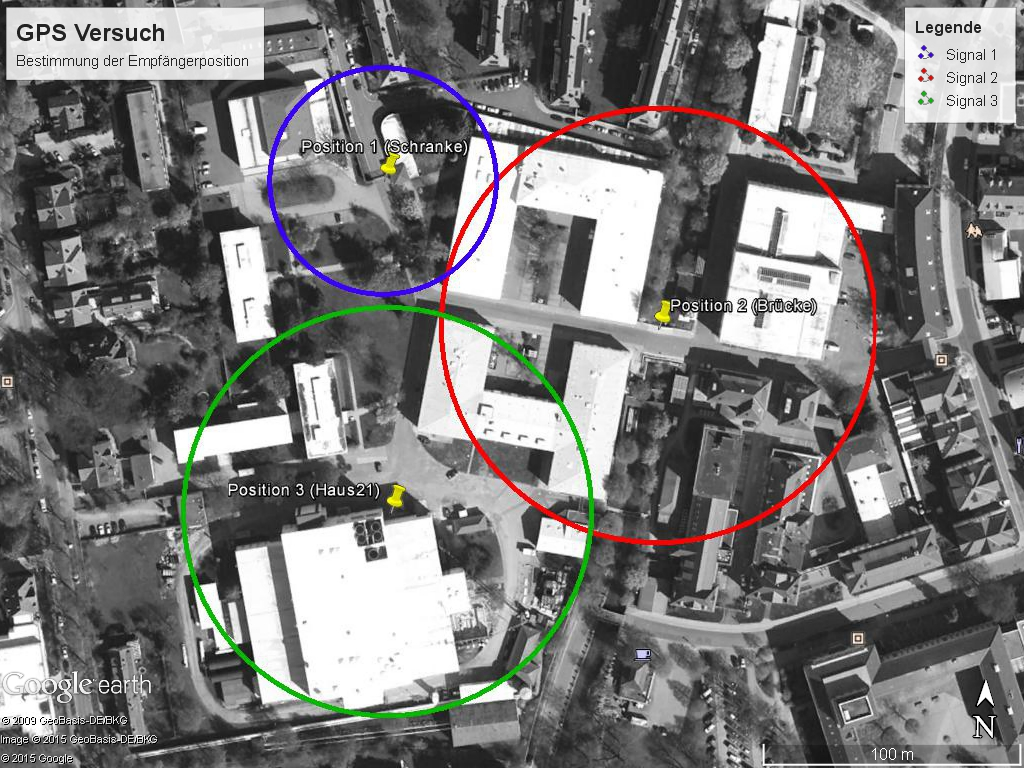
\includegraphics[width=0.8\textwidth]{GPS.jpg}
\caption{Laufzeitkreise und Startpositionen der einzelnen Signale. Wie man erkennen kann, schneiden sich die Kreise nicht, allerdings liegt in der Mitte des Raums zwischen den Kreisen der Ort des Ziels.}
\label{fig:GPS}
\end{figure}
Dieses Verfahren wird im Experiment auf kürzere Entfernungen und mit langsameren Signalen angewendet.
Drei Experimentatoren stellen sich an drei verschiedene Positionen, von denen aus sie alle das gleiche Ziel sehen können.
Sobal sie losgehen, notieren sie sich die aktuelle Uhrzeit.
Dazu ist es sinvoll, dass alle die gleiche Zeit verwenden, z.B. eine Internetseite mit der Atomuhrzeit.
Der Experimentator im Ziel schreibt sich jeweils die Ankunftszeiten auf.
Aus diesen beiden Zeiten kann der Laufzeitunterschied berechnet werden.
Zum Schluss muss nur noch die Laufgeschwindigkeit der Signale ermittelt werden.
Dies geschieht bei einer Zeitnahme über eine feste Strecke.
Kennt man die Startpositionen kann jetzt anhand des Schnittpunktes der Laufzeitkreise der Ort des Ziels errechnet werden.
Die errechneten Laufzeitenkreise sind in der Abbildung \ref{fig:GPS} zu sehen.
Wie man erkennen kann schneiden sich die Kreise nicht.
Aber in der Mitte des Raumes zwischen den Kreise liegt das Ziel.
Dies liegt zum einen an zu ungenauen bzw. zu langsamen gemessenen Geschwindigkeiten der Signale bei der Geschwindigkeitsmessung.
Zum anderen aber auch daran, dass einige der Signale keinen ebenen Weg zurück gelegt haben.
Speziell das Signal von der Brücke hatte fast einen Meter Höhenunterschied, was sich auch in der starken Abweichung zum Zielpunkt zeigt.

\section{Foucaultsches Pendel}

\subsection{Theorie}
Das Foucaultsche Pendel ist ein Schwerependel.
Für dieses ist die tangentiale Komponente der Schwerkraft die einzige Rückstellkraft.
Für diese Gilt nach Newton $F_\text{tan}=mg\sin{\varphi(t)}$.
Für kleine Winkel kann der Sinus auch linear genähert werden.
Zu dem lässt sich die Tangentialbeschleunigung mithilfe der Länge in eine Winkelbeschleunigung umrechnen.
Hieraus ergibt sich eine Differentialgleichung
\begin{align*}
	ml\ddot{\varphi}=mg\varphi.
\end{align*}
Die Lösung der Differentialgleichung $\varphi(t)=A\cdot\sin{\omega\cdot t}$ ergibt sich durch einen Exponentialansatz und Lösen der Eigenwertgleichung.
Hierbei ist $A$ die Amplitude der Schwingung und
\begin{align*}
	\omega=\sqrt{\frac{g}{l}}
\end{align*}
die Frequenz der Schwingung.
Aus dieser lässt sich die Periodendauer 
\begin{align}
	T=2\pi\sqrt{\frac{l}{g}}\label{eq:periode}
\end{align}
bestimmen.
Diese ist somit nicht von der Masse des Pendel abhängig.\\
Das Foucaultsche Pendel besitzt eine weitere Frequenz, da es sich im Laufe des Tages einmal um die eigene Achse dreht und somit einen Kreis beschreibt.
Dies gilt aber nur für ein Pendel, das auf der Drehachse der Erde aufgehängt ist.
Bewegt man sich mit dem Pendel weiter gegen Äquator, so wird die Periodendauer für den ganzen Kreis immer Länger, bis sie zum Äquator hin gegen $\infty$ strebt.
Dies ergiebt sich aus
\begin{align}
	\omega=&\omega_E\sin{\Phi}, \text{bzw.}\\
	T=&\frac{24\si{\hour}}{\sin{\Phi}}\label{eq:peri}
\end{align}
und ist vom Winkel $\Phi$ bezüglich des Äquators abhängig.
Der Breitengrad von Göttingen ist $51.53\si{\degree}$.


\subsection{Experiment kleines Pendel}
\begin{figure}[!h]
\centering
% GNUPLOT: LaTeX picture with Postscript
\begingroup
  \makeatletter
  \providecommand\color[2][]{%
    \GenericError{(gnuplot) \space\space\space\@spaces}{%
      Package color not loaded in conjunction with
      terminal option `colourtext'%
    }{See the gnuplot documentation for explanation.%
    }{Either use 'blacktext' in gnuplot or load the package
      color.sty in LaTeX.}%
    \renewcommand\color[2][]{}%
  }%
  \providecommand\includegraphics[2][]{%
    \GenericError{(gnuplot) \space\space\space\@spaces}{%
      Package graphicx or graphics not loaded%
    }{See the gnuplot documentation for explanation.%
    }{The gnuplot epslatex terminal needs graphicx.sty or graphics.sty.}%
    \renewcommand\includegraphics[2][]{}%
  }%
  \providecommand\rotatebox[2]{#2}%
  \@ifundefined{ifGPcolor}{%
    \newif\ifGPcolor
    \GPcolortrue
  }{}%
  \@ifundefined{ifGPblacktext}{%
    \newif\ifGPblacktext
    \GPblacktexttrue
  }{}%
  % define a \g@addto@macro without @ in the name:
  \let\gplgaddtomacro\g@addto@macro
  % define empty templates for all commands taking text:
  \gdef\gplbacktext{}%
  \gdef\gplfronttext{}%
  \makeatother
  \ifGPblacktext
    % no textcolor at all
    \def\colorrgb#1{}%
    \def\colorgray#1{}%
  \else
    % gray or color?
    \ifGPcolor
      \def\colorrgb#1{\color[rgb]{#1}}%
      \def\colorgray#1{\color[gray]{#1}}%
      \expandafter\def\csname LTw\endcsname{\color{white}}%
      \expandafter\def\csname LTb\endcsname{\color{black}}%
      \expandafter\def\csname LTa\endcsname{\color{black}}%
      \expandafter\def\csname LT0\endcsname{\color[rgb]{1,0,0}}%
      \expandafter\def\csname LT1\endcsname{\color[rgb]{0,1,0}}%
      \expandafter\def\csname LT2\endcsname{\color[rgb]{0,0,1}}%
      \expandafter\def\csname LT3\endcsname{\color[rgb]{1,0,1}}%
      \expandafter\def\csname LT4\endcsname{\color[rgb]{0,1,1}}%
      \expandafter\def\csname LT5\endcsname{\color[rgb]{1,1,0}}%
      \expandafter\def\csname LT6\endcsname{\color[rgb]{0,0,0}}%
      \expandafter\def\csname LT7\endcsname{\color[rgb]{1,0.3,0}}%
      \expandafter\def\csname LT8\endcsname{\color[rgb]{0.5,0.5,0.5}}%
    \else
      % gray
      \def\colorrgb#1{\color{black}}%
      \def\colorgray#1{\color[gray]{#1}}%
      \expandafter\def\csname LTw\endcsname{\color{white}}%
      \expandafter\def\csname LTb\endcsname{\color{black}}%
      \expandafter\def\csname LTa\endcsname{\color{black}}%
      \expandafter\def\csname LT0\endcsname{\color{black}}%
      \expandafter\def\csname LT1\endcsname{\color{black}}%
      \expandafter\def\csname LT2\endcsname{\color{black}}%
      \expandafter\def\csname LT3\endcsname{\color{black}}%
      \expandafter\def\csname LT4\endcsname{\color{black}}%
      \expandafter\def\csname LT5\endcsname{\color{black}}%
      \expandafter\def\csname LT6\endcsname{\color{black}}%
      \expandafter\def\csname LT7\endcsname{\color{black}}%
      \expandafter\def\csname LT8\endcsname{\color{black}}%
    \fi
  \fi
    \setlength{\unitlength}{0.0500bp}%
    \ifx\gptboxheight\undefined%
      \newlength{\gptboxheight}%
      \newlength{\gptboxwidth}%
      \newsavebox{\gptboxtext}%
    \fi%
    \setlength{\fboxrule}{0.5pt}%
    \setlength{\fboxsep}{1pt}%
\begin{picture}(7200.00,5040.00)%
    \gplgaddtomacro\gplbacktext{%
      \csname LTb\endcsname%
      \put(946,704){\makebox(0,0)[r]{\strut{}$9.4$}}%
      \put(946,1286){\makebox(0,0)[r]{\strut{}$9.5$}}%
      \put(946,1867){\makebox(0,0)[r]{\strut{}$9.6$}}%
      \put(946,2449){\makebox(0,0)[r]{\strut{}$9.7$}}%
      \put(946,3030){\makebox(0,0)[r]{\strut{}$9.8$}}%
      \put(946,3612){\makebox(0,0)[r]{\strut{}$9.9$}}%
      \put(946,4193){\makebox(0,0)[r]{\strut{}$10$}}%
      \put(946,4775){\makebox(0,0)[r]{\strut{}$10.1$}}%
      \put(1078,484){\makebox(0,0){\strut{}$0.5$}}%
      \put(1794,484){\makebox(0,0){\strut{}$0.6$}}%
      \put(2509,484){\makebox(0,0){\strut{}$0.7$}}%
      \put(3225,484){\makebox(0,0){\strut{}$0.8$}}%
      \put(3940,484){\makebox(0,0){\strut{}$0.9$}}%
      \put(4656,484){\makebox(0,0){\strut{}$1$}}%
      \put(5372,484){\makebox(0,0){\strut{}$1.1$}}%
      \put(6087,484){\makebox(0,0){\strut{}$1.2$}}%
      \put(6803,484){\makebox(0,0){\strut{}$1.3$}}%
    }%
    \gplgaddtomacro\gplfronttext{%
      \csname LTb\endcsname%
      \put(176,2739){\rotatebox{-270}{\makebox(0,0){\strut{}g [$\si{\meter\per\second^2}$]}}}%
      \put(3940,154){\makebox(0,0){\strut{}Länge [m]}}%
      \csname LTb\endcsname%
      \put(4114,1097){\makebox(0,0)[r]{\strut{}Messwerte}}%
      \csname LTb\endcsname%
      \put(4114,877){\makebox(0,0)[r]{\strut{}$\bar{g}=(9.83\pm0.08) \,\si{\meter\per\second^2}$}}%
    }%
    \gplbacktext
    \put(0,0){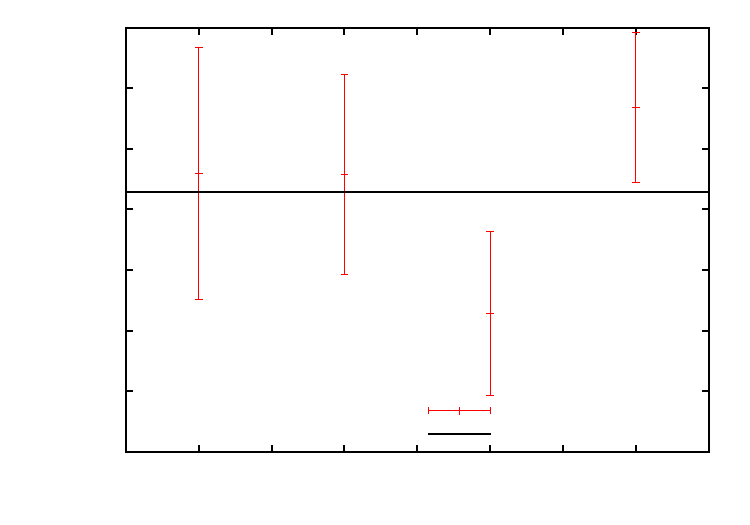
\includegraphics{gbesch}}%
    \gplfronttext
  \end{picture}%
\endgroup

\caption{Erdbeschleunigung aus den gemessenen Perioden und Pendellängen. Es ist zu dem der Mittelwert als Gerade eingetragen.}
\label{fig:g}
\end{figure}
Aus einem kleinen Pendel soll die Erdbeschleunigung $g$ mithilfe der Formel \eqref{eq:periode} bestimmt werden.
Dazu werden für verschiedene Pendellängen die Perioden gemessen und in die zugehörige Erdbeschleunigung umgerechnet.
Die ermittelten Werte sind in der Abbildung \ref{fig:g} zu sehen.
Zu den Werten ist auch der Mittelwert in die Abbildung eingetragen.
Der Realwert beträgt $9.81\si{\meter\per\second^2}$.
Wie man erkennen kann war die Messung der Erdbeschleunigung recht genau.
Die Fehler kommen durch ungenaue Messung der Perioden zustande, da reines Augemaß verwendet wurde.

\subsection{Experiment großes Pendel}
Zur Bestimmung des Breitengrades von Göttingen wird ein großes Foucaultsches Pendel verwendet.
Bei diesem wird die Periodendauer gemessen um dann mithilfe der Gleichung \eqref{eq:peri} den Breitengrad zu bestimmen.
Bei der Messung ergab sich eine Drehung von $9\si{\degree}$ in $24\si{\minute}$.
Dies ergibt über den Dreisatz eine Periode von
\begin{align*}
	T=16\si{\hour}.
\end{align*}
Diese Zeit ist eindeutig zu kurz, da die Periode für Göttingen bei $30\si{\hour}$ liegen sollte.
Zu dem beudeutet diese Periodendauer, dass sich das Pendel nicht auf der Erde befunden haben kann, da die Periodendauer $24\si{\hour}$ nicht unterschreiten kann.\\
Die Fehlerquellen in diesem Fall sind zum einen nicht vernachlässigbare Reibungseffekte, da das Pendel schnell an Amplitude verliert.
Zum anderen aber auch eine mögliche Ellipsenförmige Bahn, die die Periode beschleunigt hat.
Dies führte zu einer zuhohen Drefrequenz.


\section{Erdumfang}
Um den Erdumfang zu Messen wird die Methode von Eratosthenes verwendet.
Bei dieser Methode wird der Winkel von Schattenwürfen an zwei verschiedenen Orten auf der Erde vermessen und aus dem bekannten Abstand der beiden Punkte kann dann das Bogensegment bestimmt werden, das sich über den Winkel erstreckt.
Dies funktioniert nur, wenn sich die beiden Orte auf dem selben Längengrad befinden, damit auch der Erdmittelpunkt mit der Ebene geschnitten wird.
Anschließend kann per drei-Satz dann der Gesamtumfang der Erde berechnet werden.
Eratosthenes hat dazu einen Brunnen bei Syenne benutzt, in dem zum längsten Tag des Jahres für einige Minuten die Sonnen Senkrecht einscheint.
Zum gleichen Zeitpunkt wurde der Winkel des Schattenwurfes am Obelisken in Alexandria gemessen.
Dieser betrug etwa $7.37\si{\degree}$.
Als letzte fehlende Größe musste der Abstand zwischen diesen beiden Orten bestimmt werden.
Dies erfolgte durch viele Läufer, welche die Beine nur für einen bestimmte Weite öffnen konnten und somit alle Schritte gleich lang waren.
Um Hindernisse zu umgehen wurden diese immer in rechten Winkeln umlaufen, damit sich keine Strecke zu dem Abstand hinzuaddiert, die durch Hindernisse verursacht wurde.
Hierzu wurde ein langes Seil verwendet, dessen Enden verknotet sind und welches mit 12, in gleichen Abständen gesetzten Knoten versehen ist.
Mit diesen 12 Knoten kann ein Rechtwinkliges Dreieck gebaut werden, wenn die beiden am rechten Winkel anliegenden Seiten aus drei und vier Knoten bestehen und die letzte Seite die verbliebenden 5 Knoten beinhaltet.
Aus dieser vorgehensweise ergab sich ein Abstand der beiden Orte von etwa $812\si{\kilo\meter}$ und damit ein Gesamtumfang von $39690\si{\kilo\meter}$.
Der echte Erdumfang liegt bei $40074\si{\kilo\meter}$ um somit nur $390\si{\kilo\meter}$ daneben.
Die lässt sich zum einen durch eine nicht ganz genaue Messung des Abstandes der beiden Orte erklären.
Allerdings wurde die Messung sehr häufig durchgeführt, sodass dieser Fehlerbeitrag eher klein ist.
Nicht zu vernachlässigen ist aber, dass Syenne und Alexandria nicht auf dem gleichen Längengrad liegen.
Um dies zu verbessern müsste man von Syenne aus auf den Breitangrad in Richtung des Längengrades von Alexandria gehen und anschließend den Weg auf dem Längengrad berechnen.
Diese Strecke stellt dann ein Stück des Erdumfangs dar.


\newpage
%\nocite{*} %sorgt dafuer, dass alles ausgegeben wird
\printbibliography[heading=bibintoc]
\end{document}
